\documentclass{scrreprt}
\usepackage[utf8]{inputenc}
\usepackage[english]{babel}
\usepackage[T1]{fontenc}
\usepackage{textcomp}
\usepackage[hidelinks]{hyperref}
\usepackage{graphicx}
\usepackage{amsmath}
\usepackage{amsfonts}
\usepackage{amssymb}
\newcommand{\matr}[1]{\mathbf{#1}}
\newcommand{\transpose}[1]{#1^\intercal}
\newcommand{\degr}{\text{\textdegree}}

\setcounter{secnumdepth}{5} 

\title{Camera grid extrinsic self-calibration}
\author{Tim Lenertz}
\date{\today}

\begin{document}

\maketitle

\tableofcontents

\chapter{Introduction}
This report describes the method used to calibrate the extrinsic camera parameters of the 3DLicorneA data sets. If is applicable for dense 2D data sets, where cameras are placed on a more or less regular grid on a plane parallel to the scene. The optical flow of tracked features, and aggregated values from the depth maps, are used to compute the camera positions and orientations. No calibration pattern needs to be present in the scene.

\section{Requirements}
To use the method, there are the following requirements:
\begin{itemize}
\item The intrinsic camera parameters are known. This is the camera matrix $K$ and optionally the distortion coefficients. The method was used for the case where there is no distortion (Kinect v2), but with additional steps it can be used with distorted images.
\item The intrinsic camera parameters are the same for each image.
\item There is a depth map for all or some views. There is an extension to use the method without depth maps, and instead giving a depth only for some feature points.
\item The camera centers are arranged on an approximately regular 2D grid on a plane $P$. The distance between adjacent camera positions (in X and Y direction) is sufficiently small that feature points can be tracked using optical flow. For this disparities of features on adjacent views should be smaller than 15 pixels.
\item It is assumed that camera centers lie always exactly on the plane. That is, they never more towards or back from the scene. 
\item The camera is facing approximately perpendicular to the plane $P$, towards the scene. There can be a small rotation $\matr{R}$ of the camera relative to $P$. It is estimated from the images, as part of the calibration. The yaw, pitch and roll angles should be smaller than 5\textdegree. It is assumed that this angle remains constant for all views.
\item There can be some missing images and depth maps in the data set.
\item It is not necessary that the tracked feature points remain visible across the whole range of views. Calibration can be done on subsets of the camera positions, and then stitched together.
\end{itemize}

The method calculates one global rotation matrix $\matr{R}$, and for each view $v$, a 2D vector $(x_v, y_v)$ of the camera center position on the plane $P$. From this it computes an extrinsic matrix $\matr{Rt}$ for each view.



\chapter{Method}
Calibration is done in four steps: (1) Compute \emph{image correspondences} using feature tracking. (2) Estimate the \emph{camera rotation} $\matr{R}$. (3) Estimate \emph{straight depths} of the tracked features, i.e. their distance to $P$. (4) Deduce camera positions.

\section{Overview}
First the algorithm selects several \emph{feature points} on one on multiple \emph{reference views}. Using optical flow, it then tracks the position of the same features on the other views.

With the pin-hole camera model, it is be possible to calculate the camera position on $P$ directly from a feature point's positions on different views, if the camera is pointing perpenticular to $P$, and the feature's distance to $P$ is known. So the algorithm first needs to estimate $\matr{R}$, and the straight depths of the features.

To calculate $\matr{R}$, two methods are used. One uses a non-linear model which estimates $\matr{R}$ only from the slope of the lines that the tracked features make when the camera moves horizontally and vertically, without knowledge of the features' depths. The other method uses the depths of the features on the different views. Both estimate a full 3D rotation matrix.

The distance of a feature to $P$ is called its \emph{straight depth}. Knowing $\matr{R}$, it can now be calculated from the feature points' depths in each view's depth map. If depth maps are not available, it is also possible to fix only the depth of one or more features, and deduce the rest from the relative scales of the different feature's disparities. 

Using $\matr{R}$ and the \emph{straight depth} of each feature, the algorithm now estimates the set of camera positions on $P$, once for each feature. The results are aggregated to find the final camera positions.

The resulting camera positions are in a coordinate system with the camera of the \emph{reference view} at origin. If multiple reference views were used in the feature tracking step, the entire procedure is repeated for each reference view, and in the end the camera positions are stitched together.



\section{Preliminaries}
The 2D dataset consists of several \emph{views}. A view $v$ consists of an image, and optionally a depth map, taken from one camera position. The views are enumerated with two integer indices $v(x,y)$. Views with the same $x$ index are (approximately) aligned vertically, views with the same $y$ index horizontally. This is relative to the camera image planes.

The goal is to estimate the position and orientation of the camera for each view, i.e. to find the extrinsic camera matrices $\matr{Rt}_v$.

If depth maps are used, they need to be in the same coordinate systems as the images. For each image pixel $(i_x,i_y)$, the value $d$ of the same pixel in the depth map needs to indicate the orthogonal distance from the camera center to that object point, orthogonal to the camera image plane. The camera matrices $\matr{Rt}_v$ will be expressed in the same unit as these depths.

 
\section{Image correspondences}
First some features $f$ are selected. They correspond to 3D points in the scene. This step aims to find for each feature $f$, the set of \emph{feature points} $p(f,v) = (x,y,d,w)$, that is the pixel coordinates $x,y$ where the feature is visible in each view $v$. This data is called the \emph{image correspondences}.

A feature point optionally also contains a depth $d$, and a weight $w$. The depth is a distance orthogonal to the camere image plane of $v$. If $\matr{R} \neq \matr{I}$, then the depths $p_{f,*}$ of the same feature for different views will be different.


\subsection{Choosing feature points}
Features are chosen by choosing feature points on a \emph{reference view}. By default the center view in the dataset is used as reference view, but there can also be multiple reference views (see later).

The chosen feature points need to be such that they are likely to remain \emph{stable} when doing feature tracking. It means that when one looks for a similar-looking nearby point on an adjacant view, it is likely to be the same scene point. An example is shown on figure \ref{fig:choosefeatures}.

\begin{figure}
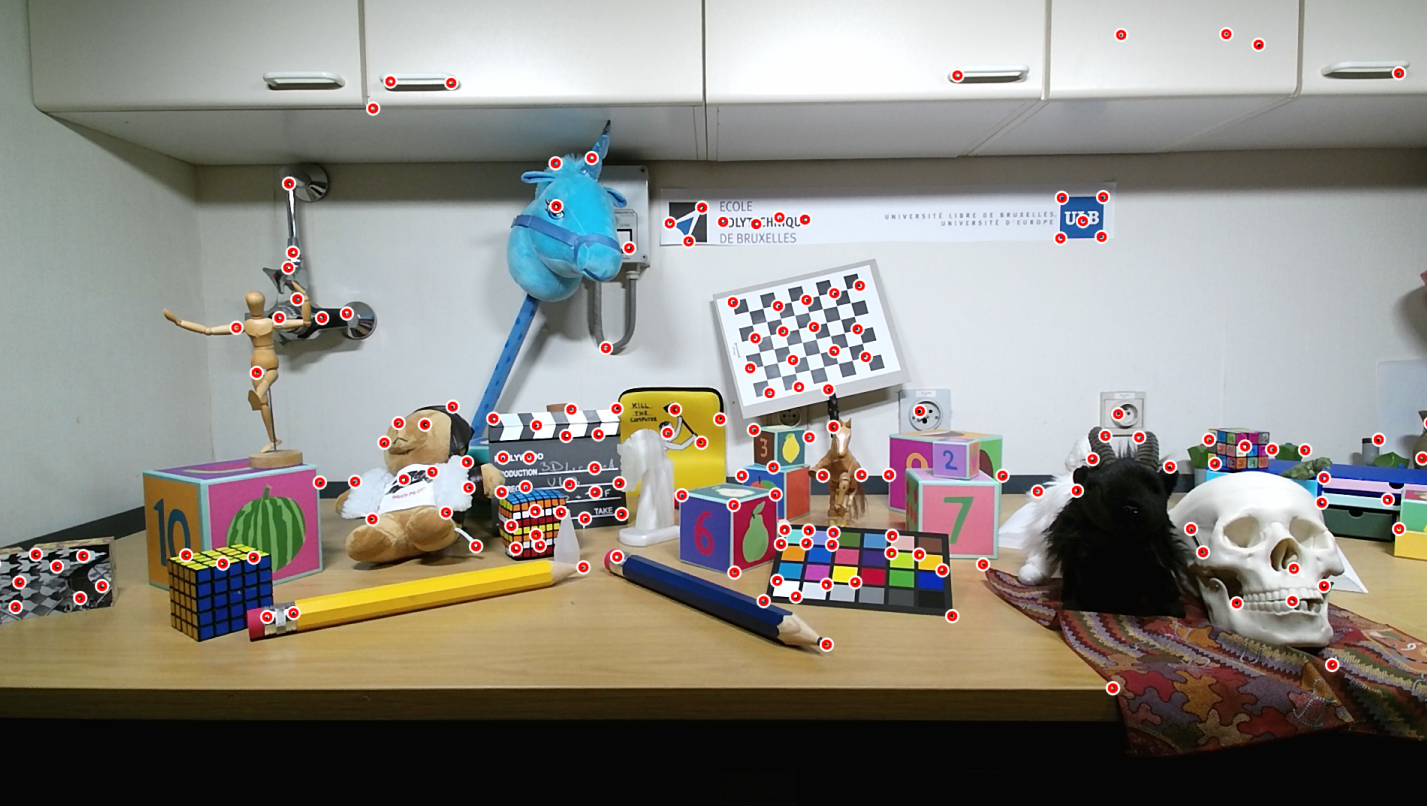
\includegraphics[width=\textwidth]{choosefeatures.png}
\caption{Chosen feature points}
\label{fig:choosefeatures}
\end{figure}

The \emph{OpenCV} function \texttt{goodFeaturesToTrack} is used. Additionally, the image is first subdivided into 4 or more rectangular regions, and the best chosen features from each region are taken.

The chosen features should be well distributed across the image, and have different depths. There should be about $300$ or more features, considering that many will be filtered out because their optical flow is unstable.


\subsection{Optical flow tracking}
Optical flow feature tracking is always done on adjacent views, for example $v(x,y)$ and $v(x+1,y)$. Then sequentially, it uses the corresponding feature points on $v(x+1,y)$ to estimate those for $v(x+2,y)$, and so on. So there is an error accumulation, which gets worse the longer the path that the view indices take is.

The acquisition system moves line-by-line. So it is physically guaranteed that for any $v(x,y)$ and $v(x+1,y)$, the camera only moves by small amount, whereas for $v(x,y)$ and $v(x,y+1)$, there can be a larger deviation. So it is better to take most optical flow correspondences in $x$ direction.


\begin{figure}
\centering
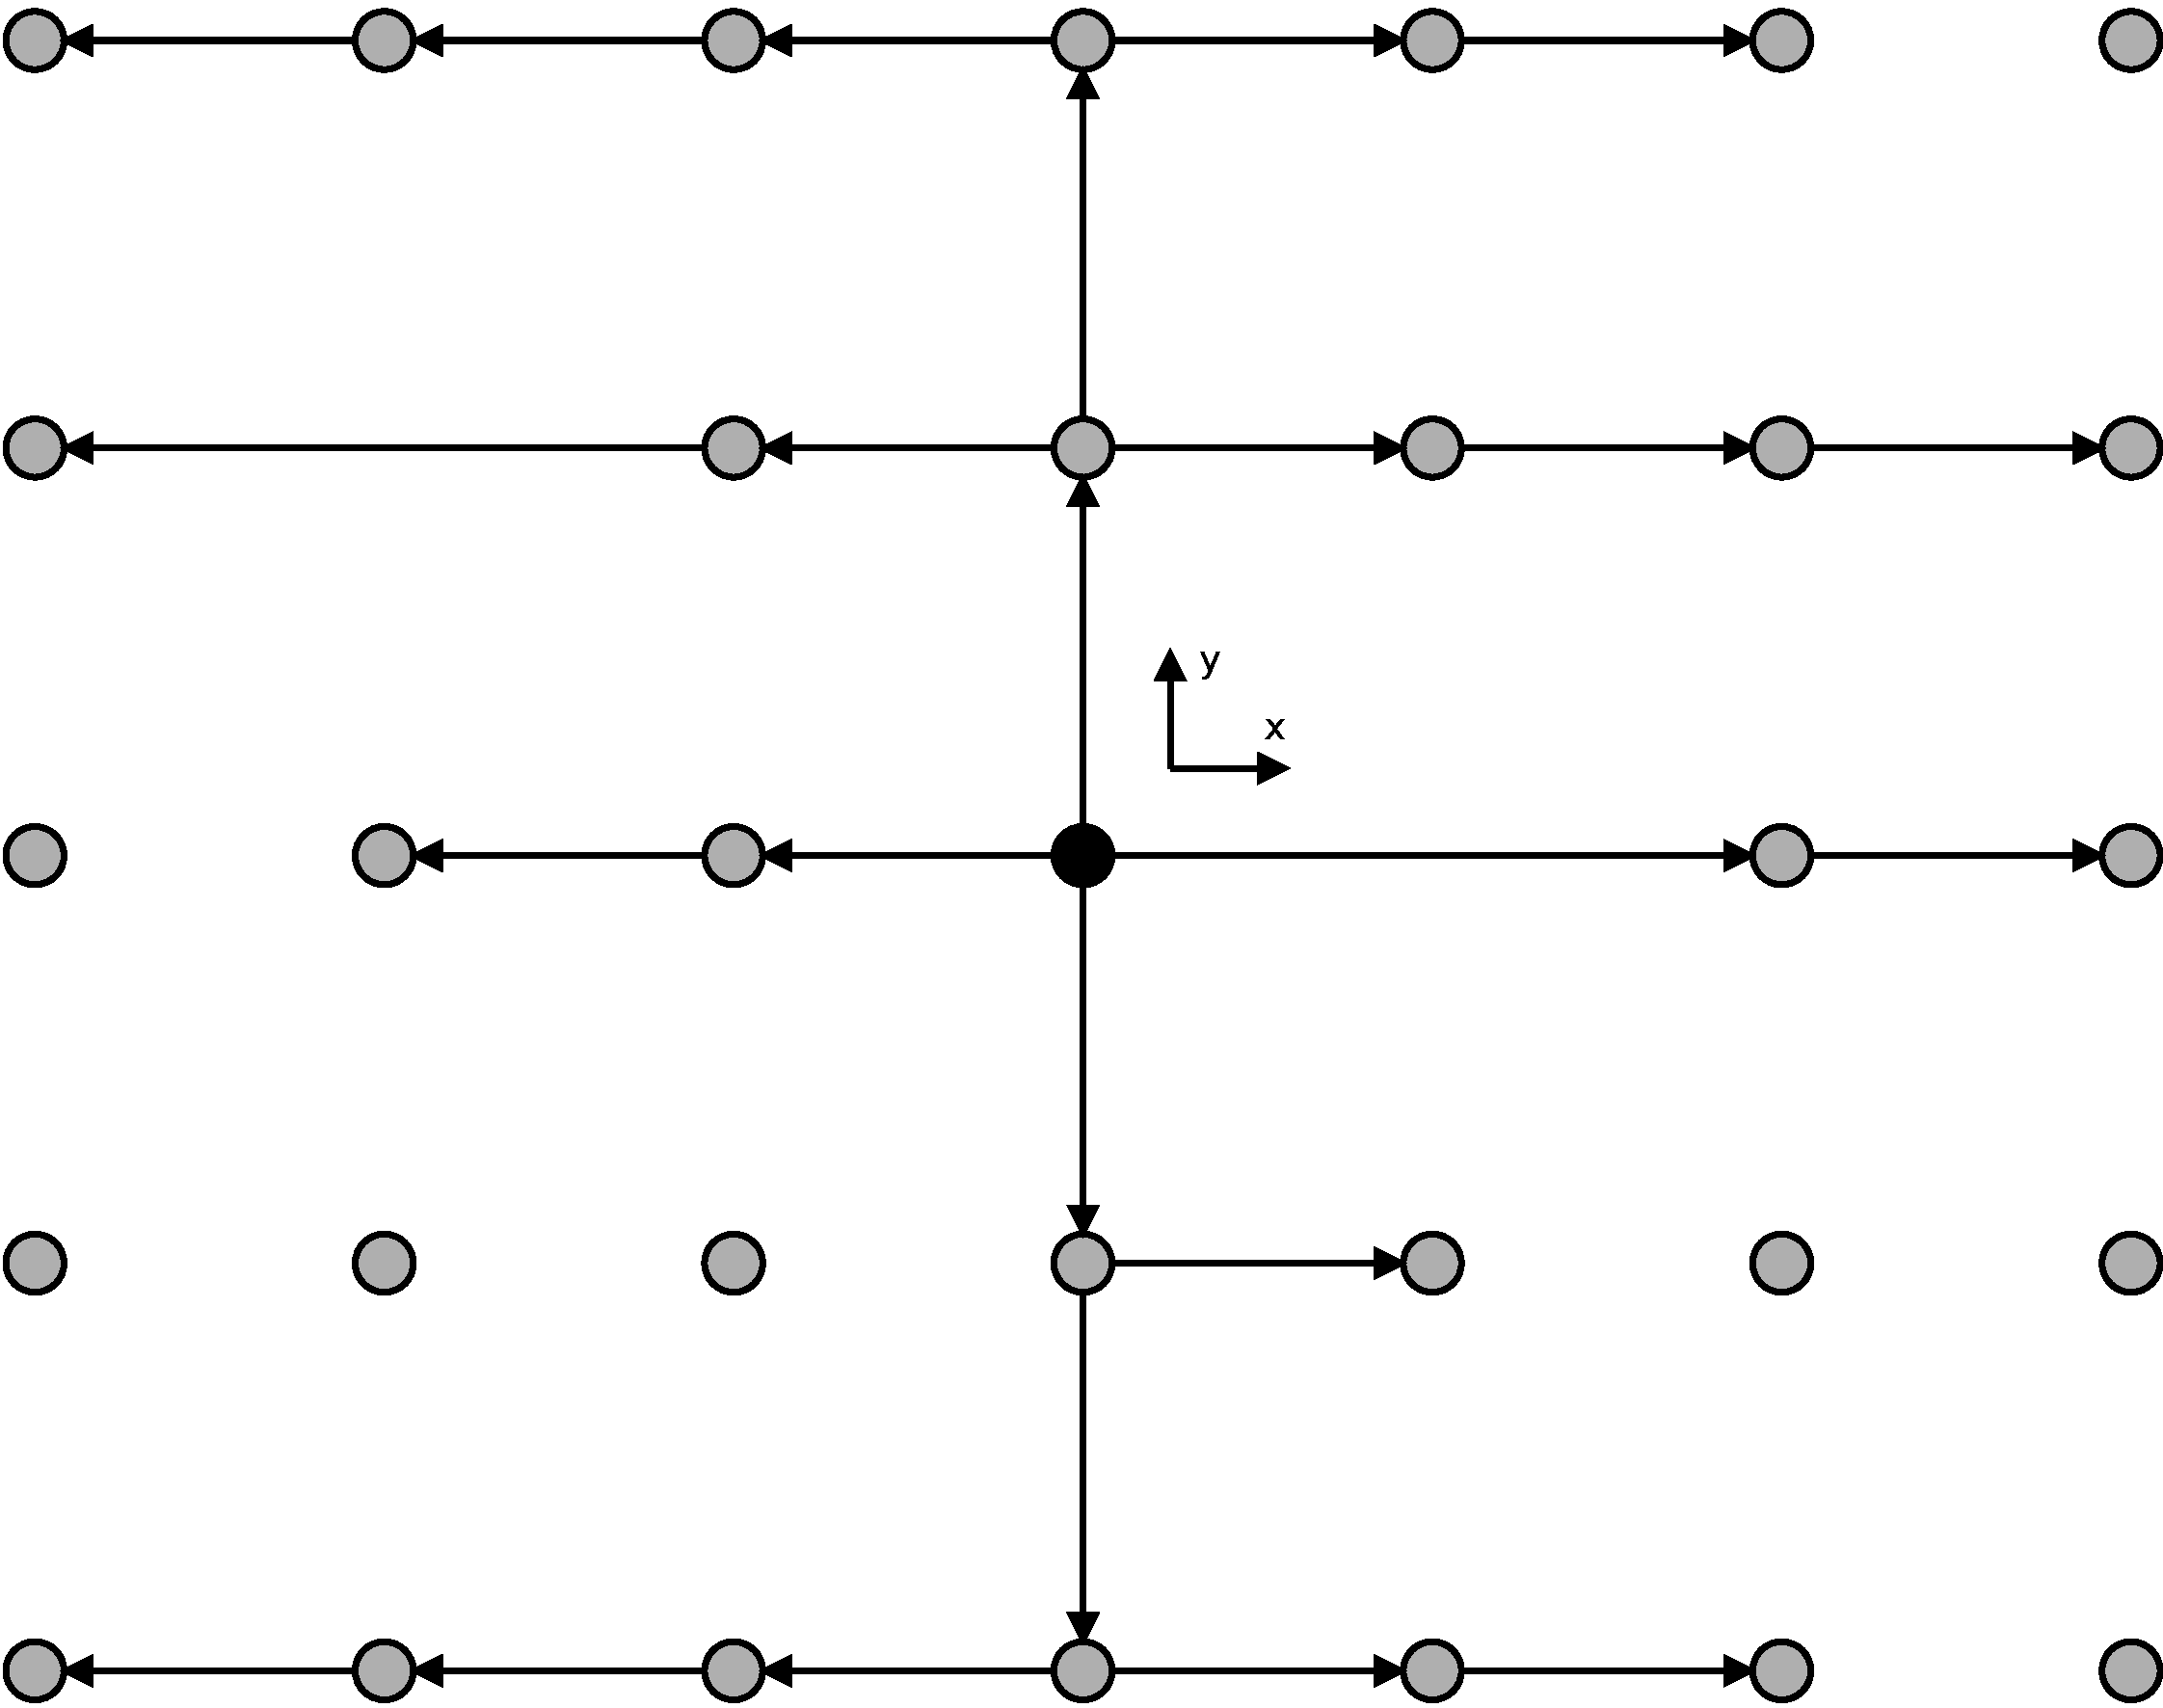
\includegraphics[width=0.6\textwidth]{opticalflow.pdf}
\caption{Optical flow paths}
\label{fig:opticalflow}
\end{figure}

The optical flow algorithm moves over the $(x,y)$ view indices as shown on figure \ref{fig:opticalflow}. The center view (black circle) is the reference view. As each step moving from $(x,y)$ to $(x',y')$, for each feature $f$, all the feature points $p(f,v(x',y'))$ are computed from those of $p(f,v(x,y))$. If no feature point $p(f,v(x',y'))$ could be computed anymore, the algorithm stops for that line.

If the image for a view is missing, that view is skipped, and instead the correspondences are taken from the second-previous view, as shown. It is important that no view is missing in the column of the reference view, because then that entire line will be skipped.

The reference view is not one of the edges, but instead in the center, and the optical flow steps are done in all four directions. This minimizes the total path taken, and reduces the accumulated error.

The maximal number of steps to be taken in $x$ and in $y$ direction, called \emph{outreach}, can be set to a maximal limit. Using a smaller \emph{outreach}, and instead doing the calibration from multiple reference views, and combining the results in the end, can produce better final results.

To compute the optical flow, the \emph{OpenCV} function \texttt{calcOpticalFlowPyrLK} is used. The parameters can be adjusted. It can also be set to use multi-scale image pyramids, so that larger features can be used.

\begin{figure}
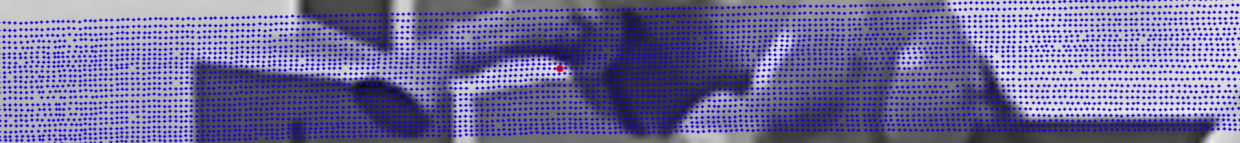
\includegraphics[width=\textwidth]{ofgood1.png}
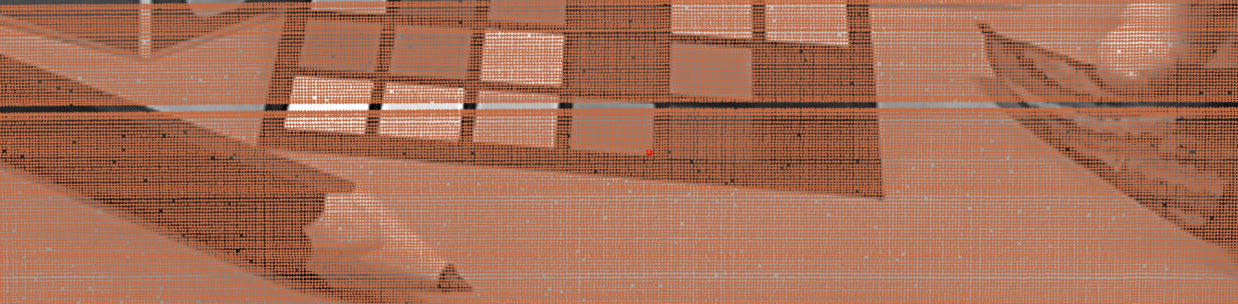
\includegraphics[width=\textwidth]{ofgood2.png}
\caption{Good feature correspondences}
\label{fig:ofgood}
\end{figure}

Figures \ref{fig:ofgood} are examples of good feature correspondences. The background image is a close-up of a view image. The red dot is the feature point on this view. The other dots are the corresponding feature points on the other views. 

\subsection{Filtering features}
The next step is to filter the generated \emph{image correspondences}. It is important, because incorrect feature points can have a large impact on the final results. The optical flow procedure tends to generate a large number of bad correspondences. There is an algorithm to automatically filter out bad correspondences, but they should also be verified by hand.

Figures \ref{fig:ofbad} are examples of good feature correspondences. In the first example, the deviation occured because a foreground object with a curved border moved in front of the tracked feature. Such deviations can also occur because of specular reflections (for example on the metal sink), and because of badly chosen feature (such as on the furry objects). In the second example, the pattern appears regular but the correspondence is still incorrect.

The filtering algorithm removes all feature points for one a feature $f$ entirely, if there are too little feature points, or if the pattern deviates too much from a regular lattice.

Properly filtering the correspondences is important: Having incorrect correspondences, and having too little correspondences, both have a large impact on the final result. In practice, for each view, there should remain feature points for about $100$ features.

\begin{figure}
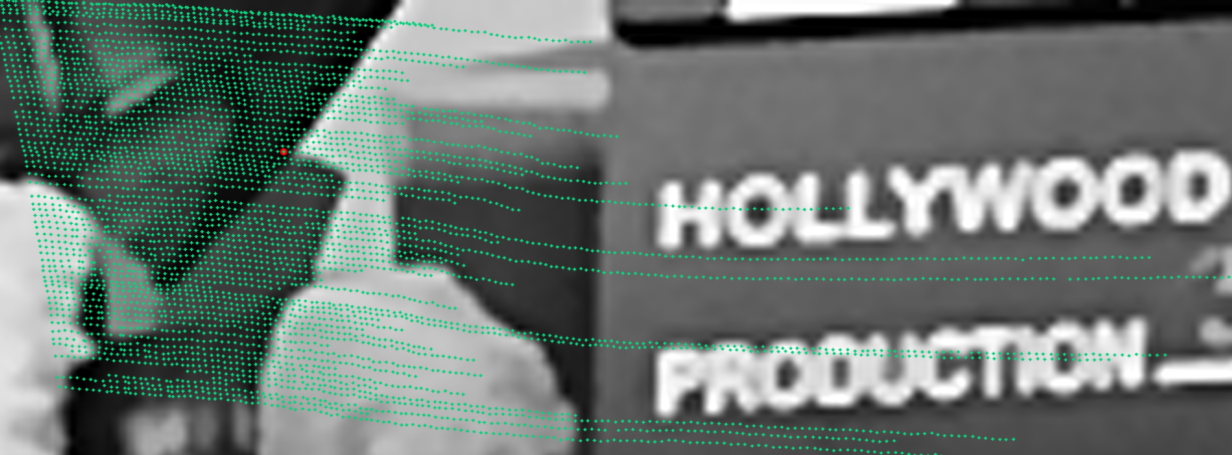
\includegraphics[width=\textwidth]{ofbad2.png}
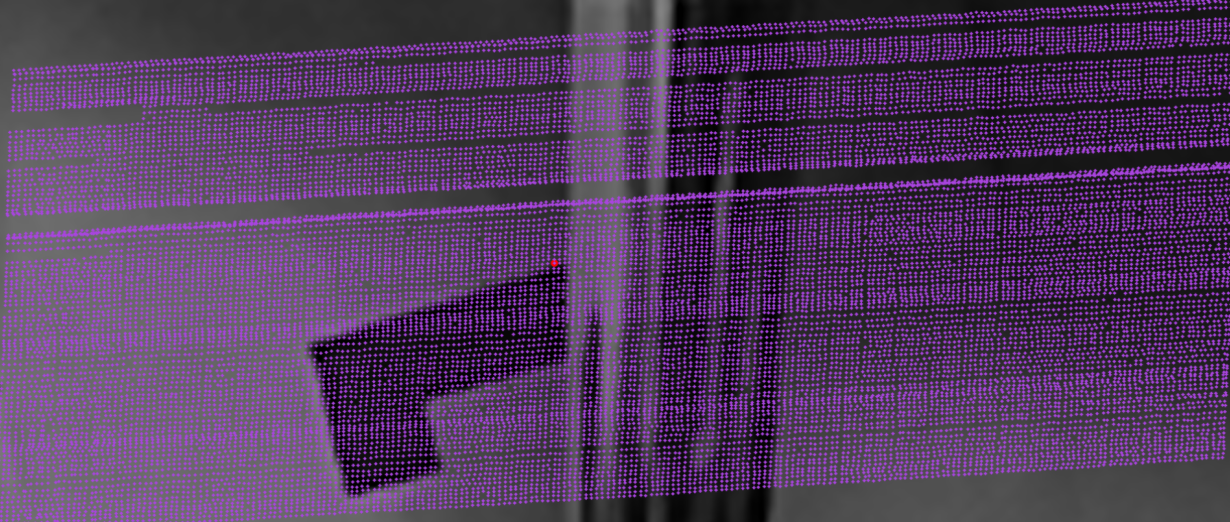
\includegraphics[width=\textwidth]{ofbad1.png}
\caption{Bad feature correspondences}
\label{fig:ofbad}
\end{figure}



\subsection{Reference views}
If the range of motion of the camera is large, or the field of view is small, many feature points that are visible in the center view, will not be visible on the extremity views. Also as said before it can be good to limit the optical flow \emph{outreach}, so as to reduce the accumulated error.

When multile reference views are used, the entire calibration will be done for each reference view independently (except for the rotation estimation, as $\matr{R}$ is constant).

Figure \ref{fig:refview} shows how reference views can be selected. The four colored dots are the reference views. They must be selected so that they are in a grid, for the stitching algorithm to work later. It is called the \emph{reference grid}. The \emph{x key} and \emph{y key} is the distance between reference view indices, in $x$ and $y$ direction.

In the figure, the outreach is set so that for feature points chosen for one reference view, correspondences can only be found for views within the same-colored rectangle. For the stitching to work, there must be some overlap in these rectangles, as shown by the yellow regions in the figure. 

The overlap should be large enough so that there will remain many views with feature points from two references, after the filtering.

For example an \emph{outreach} of $80$, and a \emph{key} of $100$ can be a good choice. It would leave an overlap range of $60$.

The algorithm chooses the \emph{reference grid} so that there are no missing images on the columns of the reference views' $x$ indices.

\begin{figure}
\centering
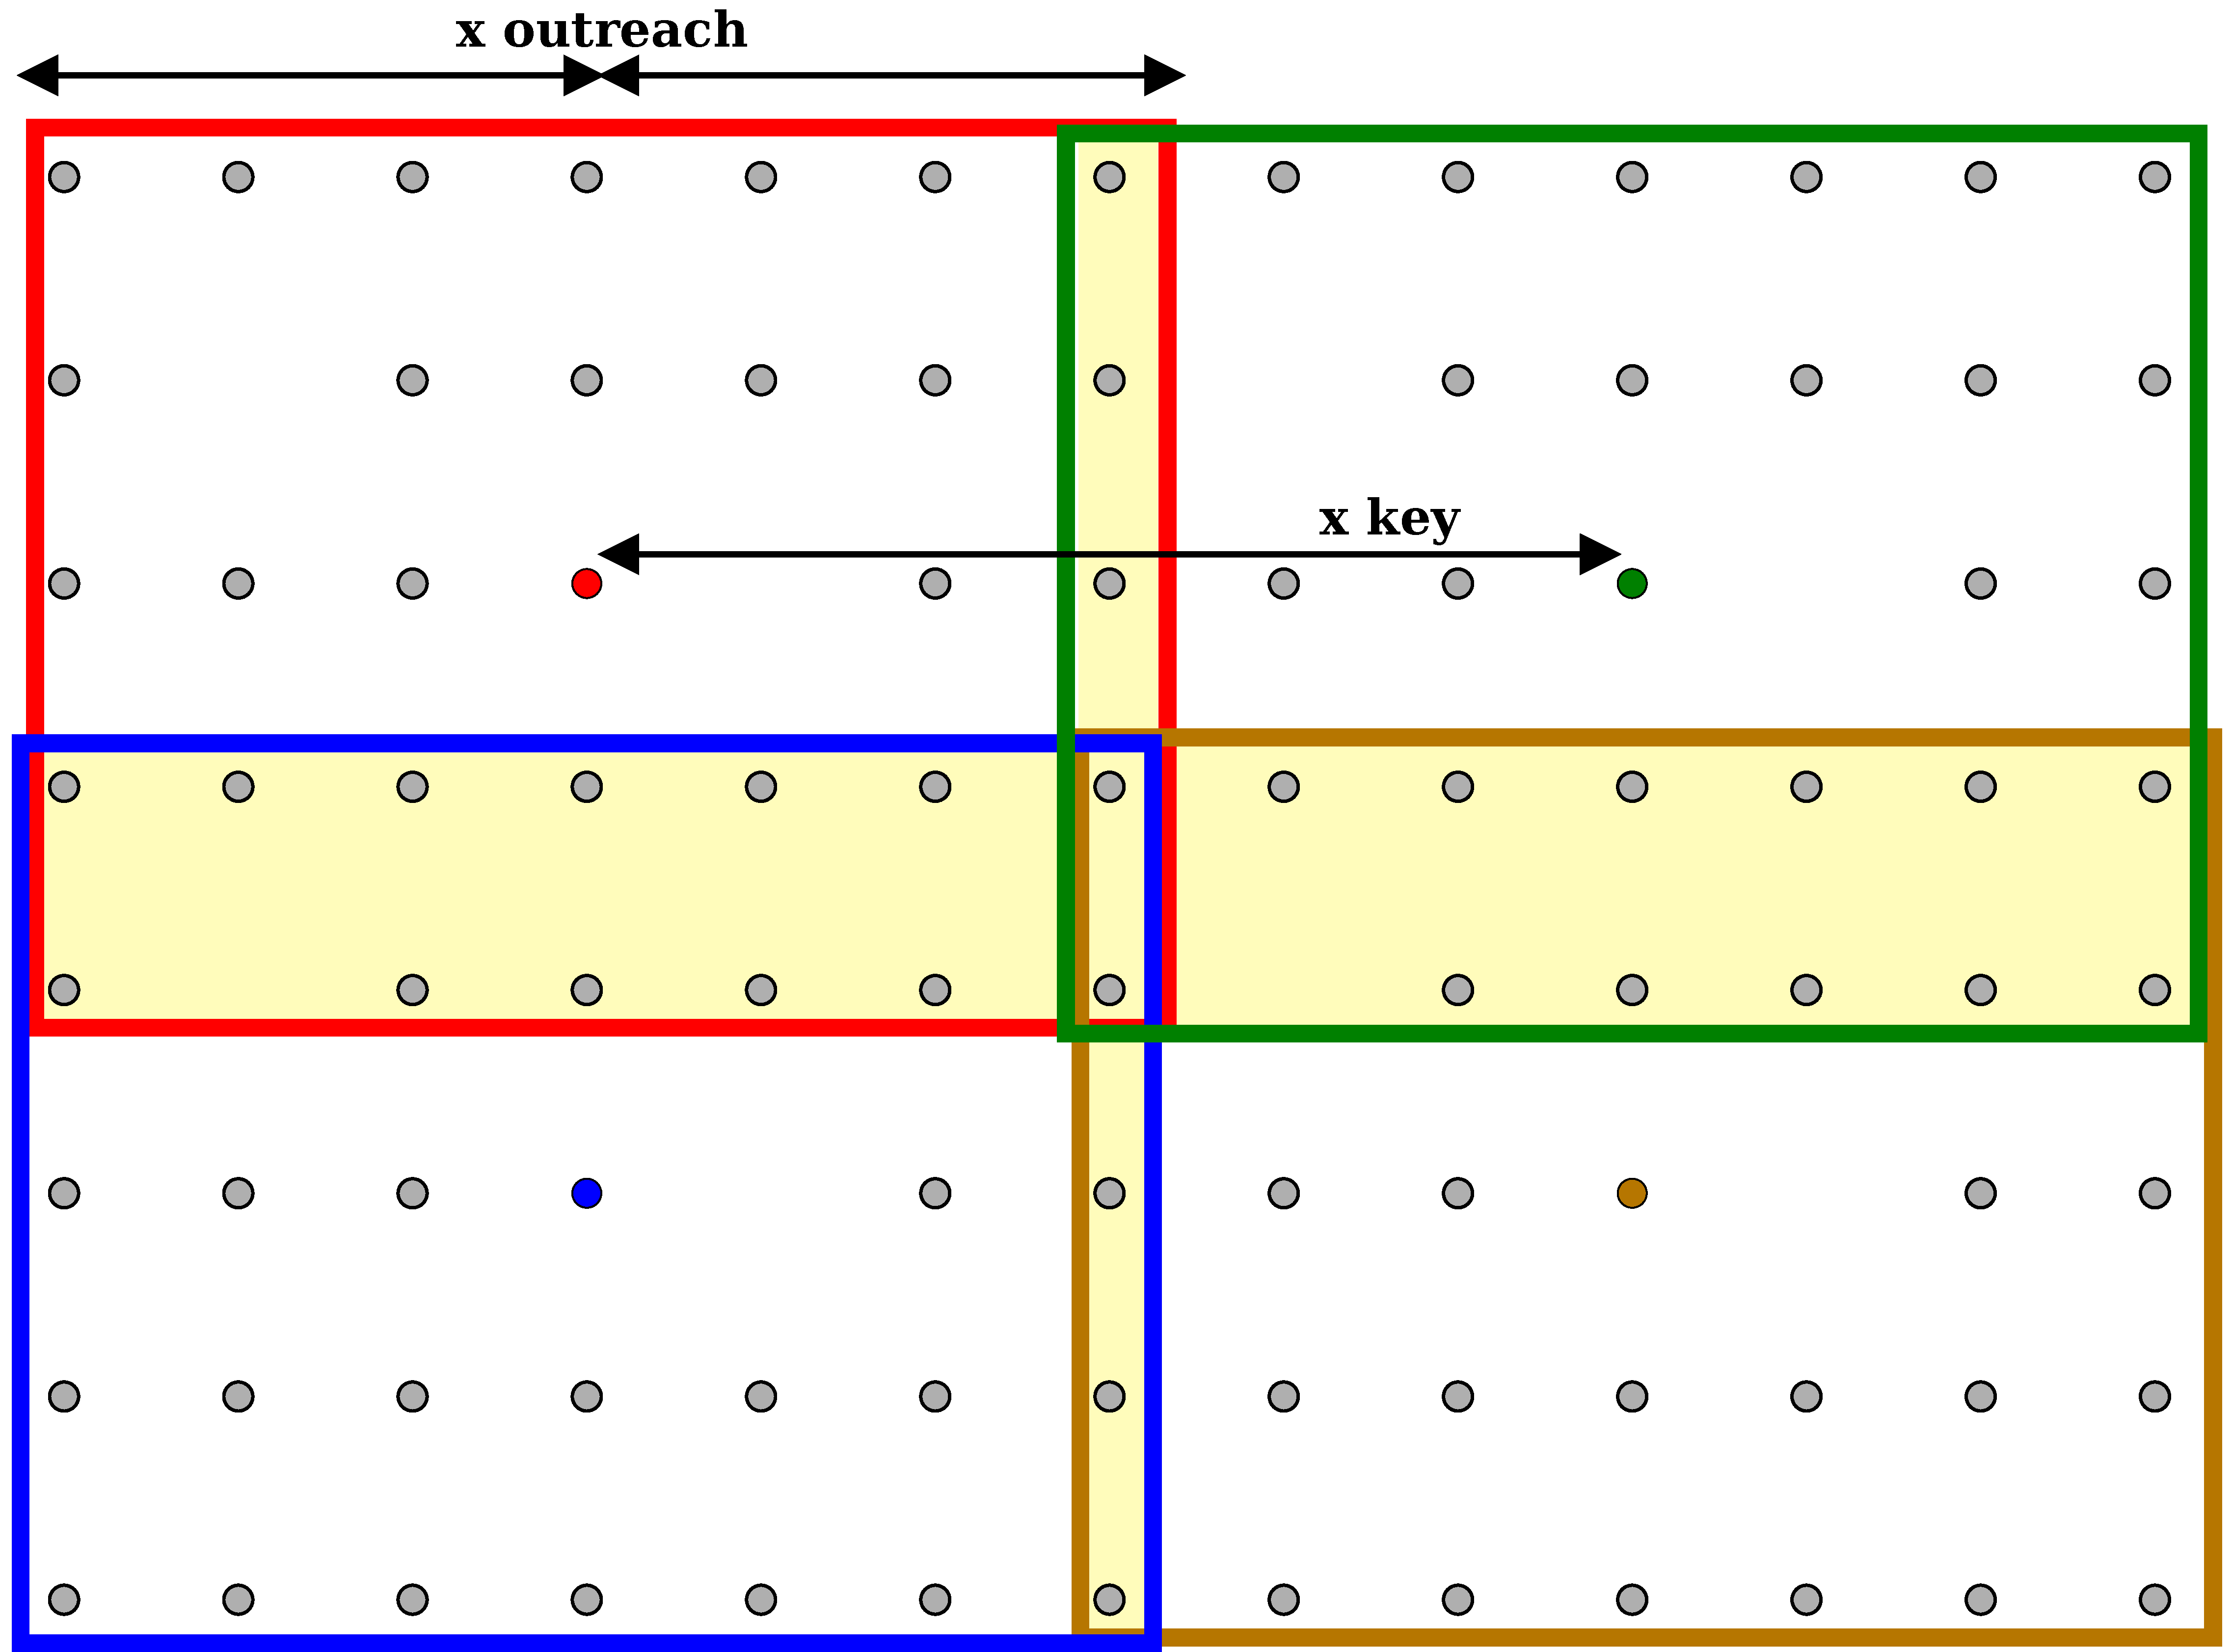
\includegraphics[width=0.8\textwidth]{refview.pdf}
\caption{Reference views arrangement}
\label{fig:refview}
\end{figure}


\subsection{Feature point depths}
If depth maps are available, they are used to attribute a depth value $d$ to each feature point $p(f,v) = (x,y,d,w)$. The depth is read from the view's depth map, at pixel position $(x,y)$.

However, features are often located on the border of foreground objects. Taking a single pixel value in the depth map could incorrectly take the depth of the background, or an incorrect intermediary value. Therefore the algorithm takes a small pixel window around $(x,y)$, and retains the minimal value in it.



\subsection{Feature point weights}
Feature points $p(f,v)$ can have a weight value. If many feature points are clustered together on a small region of the image (for example a checkerboard), it is reasonable to given them a lower weight, and to give a higher weight to more isolated feature points. The weight could also depend on a confidence value calculated for the correspondence.

Especially for the rotation estimation from optical flow slopes (see later), it is important that all regions in the image are uniformly represented.

This is not implemented.

\pagebreak
\section{Observations}
Looking at the image correspondences on figures \ref{fig:ofgood}, it can be seen that the arrangement of the feature points roughly corresponds to the (inverted) camera positions on $P$. (The vertical gap on the second figure is a result of the acquisition system: It did not take the $y$-step properly at that height.) 

The feature points for every feature $f$ will be arranged in the same pattern, just at different places in the image, and with different scales (i.e. disparities). The basic idea of this calibration method is to overlay the feature points for several features, make their scale uniform, and take the averages, to get a good estimate of the camera positions.

\begin{figure}
\centering
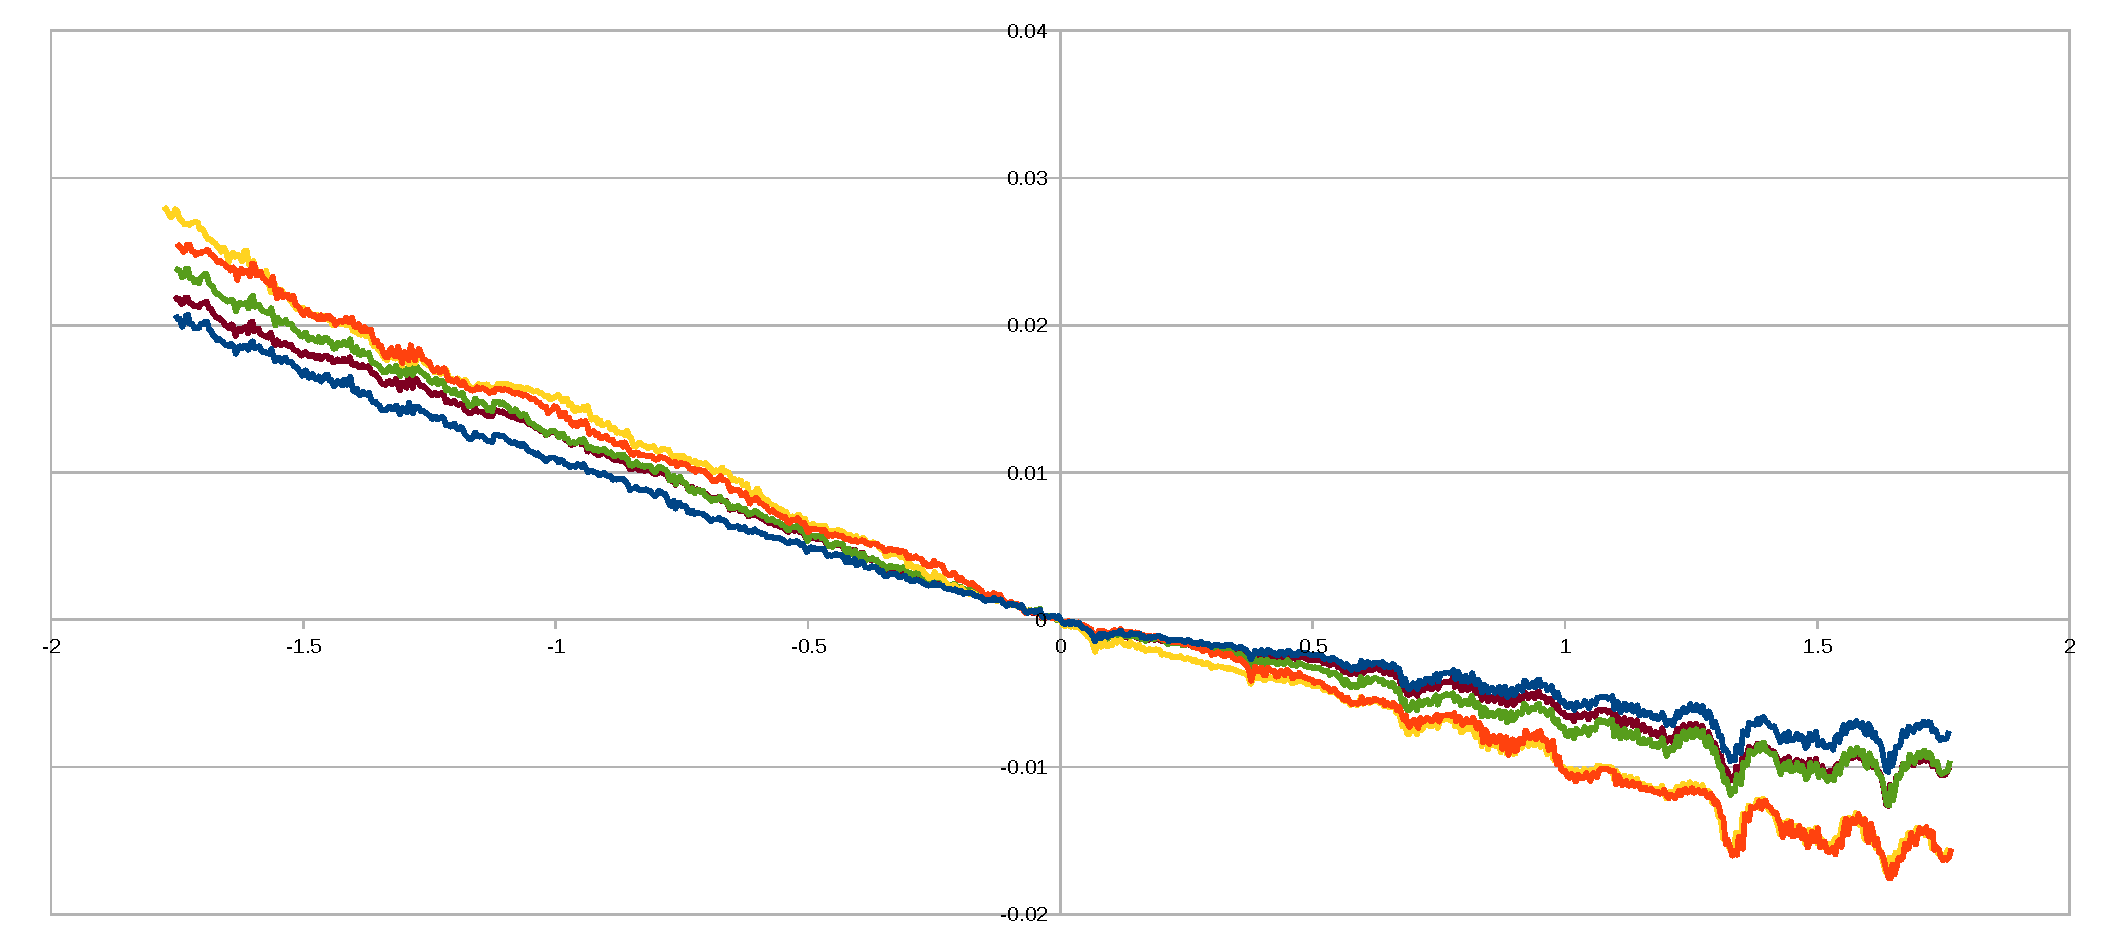
\includegraphics[width=\textwidth]{onedimslopes.pdf}
\caption{Overlayed feature points in 1D case}
\label{fig:onedimslopes}
\end{figure}

\subsection{Rotation}
However this would only be correct if $\matr{R} = \matr{I}$. In reality, the rotation $\matr{R}$ distorts the feature points. For figure \ref{fig:onedimslopes}, a 1D optical flow was taken, with the camera moving on a horizontal axis only. The feature points were then overlayed, centered on one feature point, and given uniform scale. The figure shows these transformed feature points, one color for each feature. It can be seen that they form lines with different slopes. The scaling does not affect the slope. The different slopes are caused by the camera's rotation $\matr{R}$. In the 2D case, it is possible to calculate $\matr{R}$, from these slopes alone. This is done in section \ref{sec:camrotation}.

\subsection{Depth}
Another problem is that if more than two sets of feature points should be given a common scale, one set of feature points would need to be chosen as reference. This would amplify the error in the correspondences of that particular feature. So it is better to calculate scaling factors in a more global way. This is done with the \emph{straight depths}, in section \ref{ref:straightdepths}.

\begin{figure}
\centering
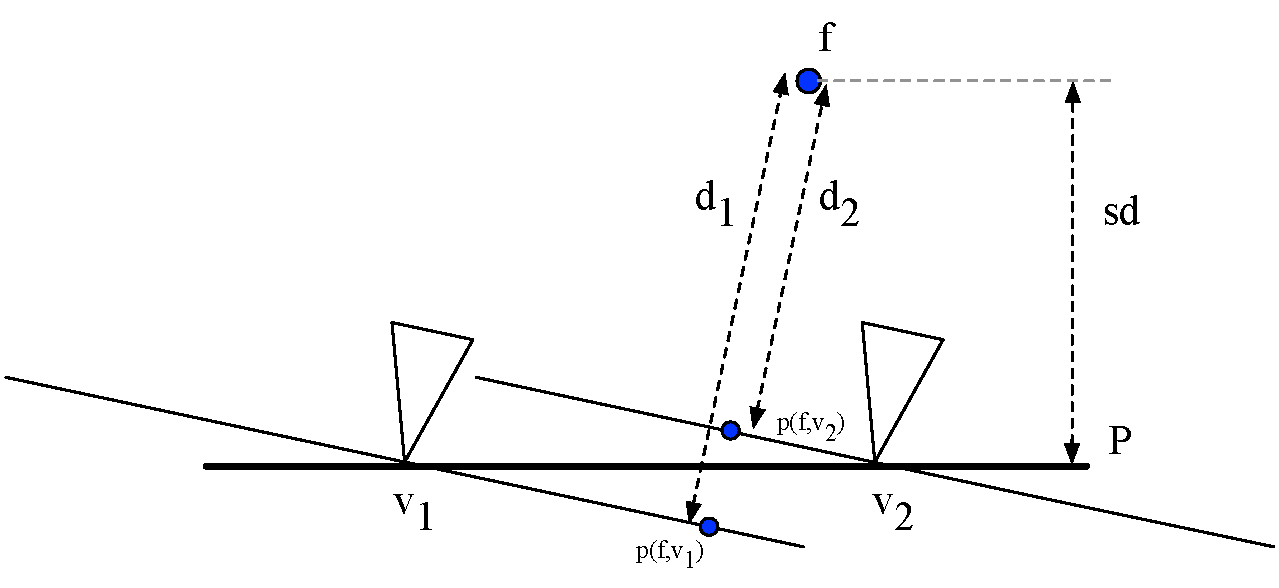
\includegraphics[width=0.7\textwidth]{differentdepths.pdf}
\caption{Differing feature point depths}
\label{fig:differentdepths}
\end{figure}

Figure \ref{fig:differentdepths} shows how because of the rotation $\matr{R}$, the feature points depths $d_1, d_2$ for one feature $f$ are not all equal. In section \ref{ref:straightdepths} all of these feature points depths are aggregated together, to calculate the straight depth $sd$, using $\matr{R}$ and the camera intrinsic matrix $\matr{K}$.



\section{Camera rotation}
\label{sec:camrotation}
The next step is to determine the camera rotation $\matr{R}$. This is the rotation of the cameras relative to the plane $P$ on which the camera centers are placed. It is a 3D rotation matrix, with 3 degrees of freedom.

If $\matr{R}$ is known to be very small, this step can be skipped entirely, by simply setting $\matr{R} = \matr{I}$.

Otherwise, there are two methods to estimate $\matr{R}$: One is based only on the \emph{slopes} of the image correspondences, and does not need depth maps. It needs the cameras to be aligned on a regular grid. It seems to produce an accuracy of around $0.5\degr$ for the three rotation angles. It is described in the next section \ref{sec:sloperot}.

The other uses the differing depths of the feature points to estimate the rotation, by doing a least squares plane fitting operation, followed by an adjustment of the roll rotation. It is described in the next section \ref{sec:depthrot}. It seems to give better results. Its implementation is only experimental, and there are probably some errors in it.


\subsection{Optical flow slopes}
\label{sec:sloperot}

\subsubsection{Flow equation}
The camera intrinsic matrix $\matr{K}$ projects points in the camera view space $(v_x, v_y, v_z)$, to pixel positions on the image $(i_x, i_y)$ in homogeneous coordinates, according to

\begin{equation}
w \begin{bmatrix}
	i_x \\ i_y \\ 1
\end{bmatrix}
= \begin{bmatrix}
	f_x & 0 & c_x \\
	0 & f_y & c_y \\
	0 & 0 & 1
\end{bmatrix}
\begin{bmatrix}
	v_x \\ v_y \\ v_z
\end{bmatrix}
\end{equation}

\begin{equation}
\label{eq:ofs_v_to_i}
i_x = f_x \frac{v_x}{v_z} + c_x
\hspace{1cm}
i_y = f_y \frac{v_y}{v_z} + c_y
\end{equation}

\begin{equation}
\label{eq:ofs_i_to_v}
v_x = \frac{v_z}{f_x} (i_x - c_x)
\hspace{1cm}
v_y = \frac{v_z}{f_y} (i_y - c_y)
\end{equation}

As shown on figure \ref{fig:differentdepths}, the camera moves such that the camera center is on a plane $P$, and the camera has a constant rotation $\matr{R}$ relative to $P$.

The \emph{world space} coordinate system is set such that its $z = 0$ plane is $P$, and its origin is any point $\vec{O}(0,0,0) \in P$.

Let $\vec{i}(\vec{O})$ be some point in the image of the camera when it is placed at $O$. Let $\vec{v}(\vec{O})$ be the same point in the camera's view space, calculated with formula \ref{eq:ofs_i_to_v}, with a given value $z = v_z(\vec{O})$. Let $\vec{w}$ be the same point in \emph{world space}. For any camera center position $\vec{Q} \in P$, the relation is
\begin{equation}
\vec{v}(\vec{Q}) = \matr{R} (\vec{w} + \vec{Q})
\end{equation}
To get from world space to view space, the coordinate system is first translated by $\vec{Q}$ (where $Q_z = 0$), then rotated by $\matr{R}$. In particular,
\begin{equation}
\vec{v}(\vec{O}) = \matr{R} \vec{w}
\end{equation}
hence
\begin{equation}
\vec{v}(\vec{Q}) = \vec{v}(\vec{O}) + \matr{R} \vec{Q}
\end{equation}
Using formula \ref{eq:ofs_v_to_i}, $\vec{i}(\vec{Q})$ can now be calculated from this. So one has the function
\begin{equation}
\text{flow}_{\matr{R}} : \langle \vec{i}(\vec{O}), \vec{Q}, z \rangle \mapsto \vec{i}(\vec{Q})
\end{equation} 

\subsubsection{Horizontal and vertical camera movement}
The following section will analyze how $\vec{i}(\vec{Q})$ evolves when $\vec{Q}$ moves on $P$. Most importantly, it is shown that when $\vec{Q}$ moves horizontally or vertically on $P$, then the \textbf{slope} at which $\vec{i}(\vec{Q})$ moves on the image does not depend on $z$.
\\ \\
Let $\vec{H} = (\epsilon,0,0)$ and $\vec{V} = (0,\epsilon,0)$. They represent a horizontal and vertical displacement of the camera on $P$, by some magnitude $\epsilon$.

Because of the transformation between cartesian and homogeneous coordinates in formulae \ref{eq:ofs_v_to_i} and \ref{eq:ofs_i_to_v}, the function $\text{flow}_{\matr{R}}$ cannot be expressed directly as a matrix equation. $\matr{R}$ is decomposed:
\begin{equation}
\matr{R} = \begin{bmatrix}
	r_{11} & r_{12} & r_{13} \\
	r_{21} & r_{22} & r_{23} \\
	r_{31} & r_{32} & r_{33}
\end{bmatrix}
\end{equation}

To simplify the expressions, the coordinates of the chosen image point $\vec{i}(\vec{O})$ are simply denoted $(i_x, i_y)$. Also, $z = v_z(\vec{O})$.

For the horizontal camera movement by $\vec{H}$, one gets:
\begin{equation}
i_x(\vec{H}) = \frac{i_x z + f_x r_{11} \epsilon + c_x r_{31} \epsilon}{z + r_{31} \epsilon}
\hspace{5mm} \text{and} \hspace{5mm}
i_y(\vec{H}) = \frac{i_y z + f_y r_{21} \epsilon + c_y r_{31} \epsilon}{z + r_{31} \epsilon}
\end{equation}

\subsubsection{Slopes}
It can be shown that as $\epsilon$ varies, $\vec{i}(\vec{H})$ moves on a straight line. Its slope is
\begin{equation}
s_H = \frac{i_x - i_x(\vec{H})}{i_y - i_y(\vec{H})}
\end{equation}
This expression simplifies to
\begin{equation}
s_H = \frac{i_x - i_x(\vec{H})}{i_y - i_y(\vec{H})} = \frac{f_y r_{21} + c_y r_{31} - i_y r_{31}}{f_x r_{11} + c_x r_{31} - i_x r_{31}}
\end{equation}
The variables $\epsilon$ and $z$ both vanish. $s_H$ depends only on $\matr{R}$, $\matr{K}$ and $\vec{i}(\vec{O})$.

For the vertical camera movement by $\vec{V}$, one gets the similar expression
\begin{equation}
s_V = \frac{i_y - i_y(\vec{V})}{i_x - i_x(\vec{V})} = \frac{f_x r_{12} + c_x r_{32} - i_x r_{32}}{f_y r_{22} + c_y r_{32} - i_y r_{32}}
\end{equation}
Note that $s_H$ is a slope $x/y$, whereas $s_V$ is a slope $y/x$. This is because $\matr{R}$ is expected to be near $\matr{I}$, and in that case $\vec{i}(\vec{H})$ and $\vec{i}(\vec{V})$ move almost horizontally and vertically on the images respectively, and so both slopes approach zero (and not infinity).


\subsubsection{Samples from image correspondences}
In order to apply this to estimate $\matr{R}$, the dataset must be such that the camera centers of views $v(x-1,y), v(x,y), v(x+1,y), \dots$ must be in an approximatly straight line (``horizontal''). For views $v(x,y-1), v(x,y), v(x,y+1), \dots$ they must also also be an approximatly straight line (``vertical''), which is perpenticular.

After the \emph{image correspondences} were computed, for each \emph{feature} $f$, a horizontal and a vertical slope $s_H(f), s_V(f)$ are estimated using line fitting on the feature point correspondences for those view indices.

This gives for each feature $f$ a sample
\begin{equation}
S_f = \langle p(f,v), s_H(f), s_V(f) \rangle
\end{equation}
$p(f,v)$ is the feature point position of $f$ for the reference view $v$. This corresponds to the $(i_x, i_y)$ from the previous formulae. If multiple reference views were used, the samples from different reference views can be put together here.


\subsubsection{Estimating camera rotation}
It is possible to estimate $\{r_{11}, r_{21}, r_{31}, r_{12}, r_{22}, r_{32}\}$ from these samples by solving two linear homogeneous least squares systems. From this $\matr{R}$ could probably be completed knowing it is an orthogonal matrix with $\det(\matr{R}) = 1$.

But this is not done in the algorithm. Instead a parameterization of $\matr{R}$ with three Euler angles $(X,Y,Z)$ is optimized with an iterative method. The error to minimize is the mean squares sum of the predicted slopes for a given $\matr{R}$, minus the measured slopes.

The parameterization $(X,Y,Z)$ of $\matr{R}$ is $\transpose{\matr{R}} = \matr{R_z}(Z) \matr{R_y}(Y) \matr{R_x}(X)$. $\transpose{\matr{R}}$ is the orientation of the camera in world space. So the \emph{roll} rotation $Z$ (around the optical axis) is performed last.

The three angles are interdependent: Say $X$ is adjusted to minimize the error. Then $Y$ is adjusted to reduce the error even more. Now $X$ is no longer at the optical setting, and needs to be readjusted.

The roll rotation has the most impact. Three golden-section searches are performed sequentially which optimize $Z$, $X$ and $Y$, in that order. The entire process is repeated iteratively until a certain error threshold. With each (outer) iteration, and tolerance and search interval of the (inner) golden-section searches are reduced.

\subsubsection{Accuracy}
On an artificially generated test dataset with a known camera rotation of $(10\degr, 20\degr, 5\degr)$, the estimated rotation was $(10.5289\degr, 20.6345\degr, 5.36933\degr)$. This artificial dataset has some random noise and outliers, $200$ features, and $30 \times 30$ views. It is hard to estimate the accuracy for real datasets because the real rotation is unknown and typically very small.

\pagebreak

\subsection{Feature point depths}
\label{sec:depthrot}



\section{Straight depths}
\label{ref:straightdepths}
Knowing $\matr{R}$, the \emph{straight depth} of each feature $f$ can now be calculated. It is the orthogonal distance of the feature point in the scene, to the plane $P$.
\subsection{Aggregating feature point depths}

\subsection{Depth from disparity}

\section{Camera positions}
Finally, having \emph{image correspondences}, the \emph{camera rotation}, and the \emph{straight depths}, the camera center positions can be computed.

\subsection{Relative camera positions}

\subsection{Stitching}

\subsection{Final camera extrinsics}

\chapter{Implementation}

 
\end{document}
